\documentclass[border=5mm,
               tikz,
               preview]{standalone}
\usetikzlibrary{arrows.meta, bending, calc, fit, positioning, shapes}

    \begin{document}
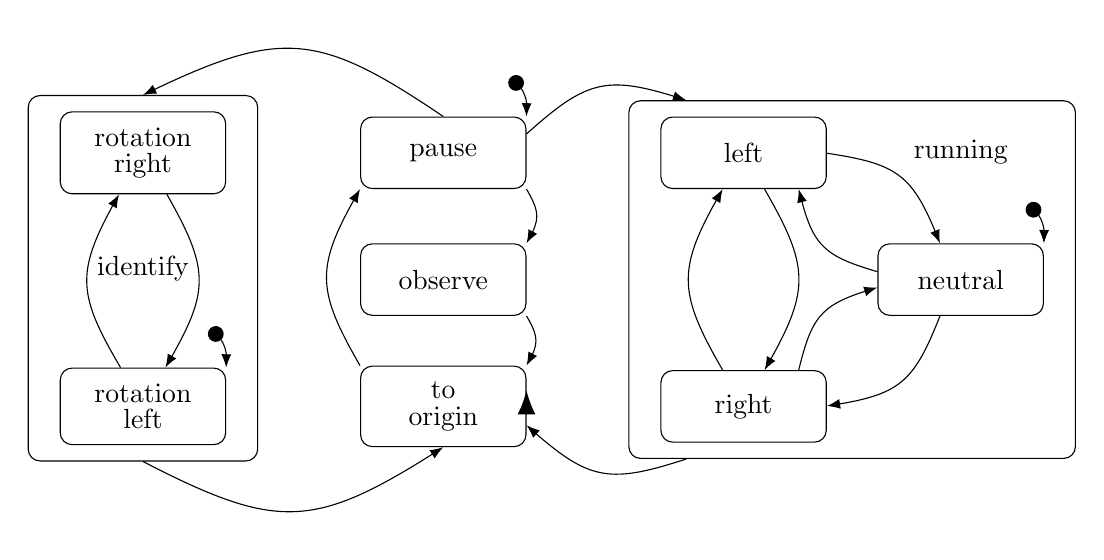
\begin{tikzpicture}[auto,
node distance = 22mm and 17mm,
every node/.style = {draw, rounded corners=1.5mm,
                     inner ysep=2mm, inner xsep=4mm,
                     minimum height=6ex,
%                     font=\bfseries,
                     text width=13mm, align=center},
                    ]
%---
\linespread{0.8}
%-------
\node (rotLeft)                             {rotation left};
\node (rotRight)    [above=of rotLeft]      {rotation right};
\node (ident)   [fit=(rotLeft)(rotRight)]   {identify};
%
\node (pause)   [right=of rotRight]          {pause};
\node (observe) [right= of $(rotLeft.east)!0.5!(rotRight.east)$]
                                            {observe};
\node (origin)  [right=of rotLeft]          {to origin};
%
\node (left)    [right=of pause]            {left};
\node (right)   [right=of origin]           {right};
\node (neutral) [right=of $(left)!0.5!(right)$] {neutral};
\node (running) [fit=(left)(right)(neutral)]    {};
    \node[draw=none,above=7mm of neutral]   {running};
%
\coordinate[above left=5mm and 2mm of rotLeft.north east]   (temp1);
\coordinate[above left=5mm and 2mm of pause.north east]     (temp2);
\coordinate[above left=5mm and 2mm of neutral.north east]   (temp3);
\path[{Circle[length=2mm,flex]}-{Latex[flex]}, bend left]
        (temp1) edge (rotLeft.north east)
        (temp2) edge (pause.north east)
        (temp3) edge (neutral.north east);
%
\draw[-{Latex[length=3mm]}]   ([yshift=-1mm] origin.east) -- + (0,3mm);
% edges
\path[draw, -{Latex[]}, bend left, looseness=1.3]
        (rotLeft)   edge (rotRight)
        (rotRight)  edge (rotLeft)
%---
        (pause.north)   edge[bend right] (ident.north) 
        (ident.south)   edge[bend right] (origin.south)
%---
        (origin.north west)     edge (pause.south west)
        (pause.south east)      edge (observe.north east)
        (observe.south east)    edge (origin.north east)
%---
        (left)      edge (right)
        (right)     edge (left)
%
        (left)      edge (neutral)
([yshift=1mm] neutral.west) edge ([xshift= 7mm] left.south)
([xshift=7mm] right.north)   to  ([yshift=-1mm] neutral.west)% exception!?
        (neutral)   edge (right)
%---
        (pause)     edge (running)
        (running)   edge (origin);
\end{tikzpicture}
    \end{document}